\documentclass[a4paper]{article}
\usepackage[utf8]{inputenc}
\usepackage[english]{babel}
\usepackage{graphicx}
\usepackage{hyperref}

\usepackage[
backend=biber,
sorting=none
]{biblatex}
\addbibresource{references.bib}

\begin{document}

\title{\Huge\textbf{MD5 Collision Attack Lab}\linebreak\linebreak\linebreak
\Large\textbf{Lab Report}\linebreak\linebreak
\linebreak\linebreak

\includegraphics[scale=0.1]{feup-logo.png}\linebreak\linebreak
\linebreak\linebreak
\Large{Integrated Master in Informatics and Computing Engineering} \linebreak\linebreak
\Large{Security in Computer Systems}\linebreak
}

\author{\textbf{Group 4:}\\
João Fidalgo - 201303098 \\
João Loureiro - 200806067 \\
Ka Chon Ho - 201711244 \\
Paulo Costa - 201206045 \\
\linebreak\linebreak
 \\ Faculdade de Engenharia da Universidade do Porto \\ Rua Roberto Frias, s\/n, 4200-465 Porto, Portugal \linebreak\linebreak\linebreak
\linebreak\linebreak\vspace{1cm}}

\maketitle

\newpage

\section{Introduction \cite{seed-labs}}

A secure one-way hash function needs to satisfy two properties: the one-way property and the collision-resistance property. The one-way property ensures that given a hash value $h$, it is computationally infeasible to find an input $M$, such that $hash(M) = h$. The collision-resistance property ensures that it is computationally infeasible to find two different inputs $M1$ and $M2$, such that $hash(M1) = hash(M2)$.

Several widely-used one-way hash functions have trouble maintaining the collision-resistance property. At the rump session of CRYPTO 2004, Xiaoyun Wang and co-authors demonstrated a collision attack against MD5 \cite{md5-col}. In February 2017, CWI Amsterdam and Google Research announced the SHAttered attack, which breaks the collision-resistance property of SHA-1 \cite{sha-1-col}. While many students do not have trouble understanding the importance of the one-way property, they cannot easily grasp why the collision-resistance property is necessary, and what impact these attacks can cause.

The learning objective of this lab is for students to really understand the impact of collision attacks, and see in first hand what damages can be caused if a widely-used one-way hash function’s collision-resistance property is broken. To achieve this goal, students need to launch actual collision attacks against the MD5 hash function. Using the attacks, students should be able to create two different programs that share the same MD5 hash but have completely different behaviors. This lab covers a number of topics described in the following:

\begin{itemize}
    \item One-way hash function
    \item The collision-resistance property
    \item Collision attacks
    \item MD5
\end{itemize}

\section{Setup}

The lab uses a tool called “Fast MD5 Collision Generation”, which was written by Marc Stevens; the name of the binary is called
\textit{md5collgen} in our demonstration.

The result of the work of Marc Stevens et al as well as the source code of the \textit{md5collgen} can be found at \href{https://www.win.tue.nl/hashclash}{https://www.win.tue.nl/hashclash}

To setup our machine we will need to download the source code for the \textit{md5collgen}, install the dependencies and compile the code. The following steps are for a Debian like system such as Ubuntu.

Download the source code with the following command:

\bigskip

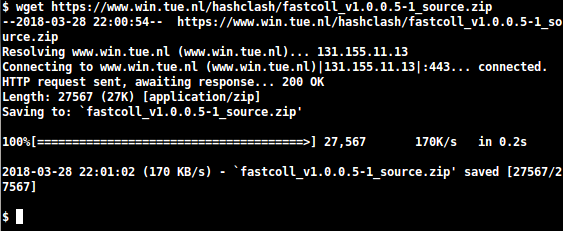
\includegraphics[width=0.9\textwidth]{bash/wget.png}

\bigskip

Then we need to extract the contents of the zip file we just downloaded.

\bigskip

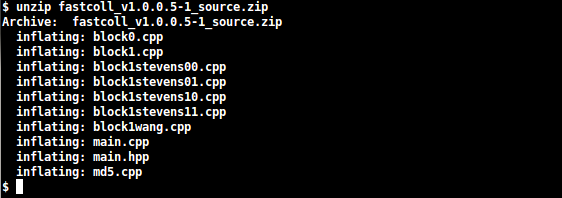
\includegraphics[width=0.9\textwidth]{bash/unzip.png}

\bigskip

Before we can compile the code we have extracted we need to install three boost libraries: \textit{system}, \textit{filesystem} and \textit{program-options}.

\bigskip

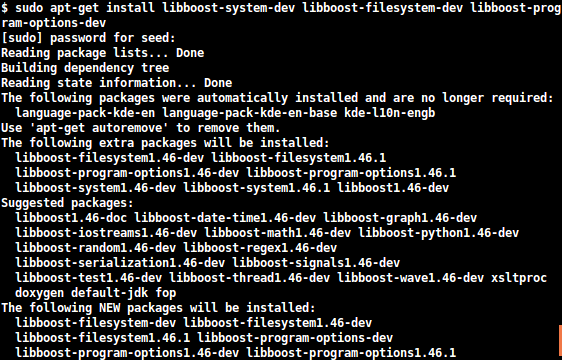
\includegraphics[width=0.9\textwidth]{bash/boost.png}

\bigskip

For the final step of our setup we need to compile the \textit{md5collgen}.

\bigskip

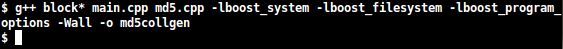
\includegraphics[width=0.9\textwidth]{bash/g++.png}

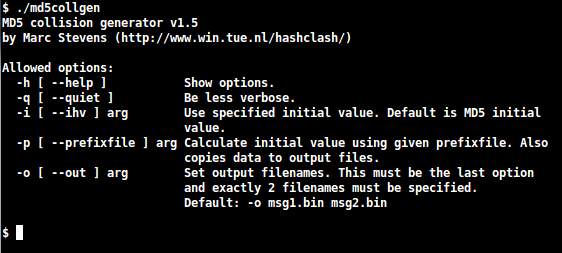
\includegraphics[width=0.9\textwidth]{bash/md5collgen.png}

\section{Lab Tasks}

\subsection{Task 1: Generating Two Different Files with the Same MD5 Hash}

\subsection{Task 2: Understanding MD5’s Property}

\subsection{Task 3: Generating Two Executable Files with the Same MD5 Hash}

\subsection{Task 4: Making the Two Programs Behave Differently}

\newpage

\printbibliography

\end{document}
